% This file was created by tikzplotlib v0.9.1.
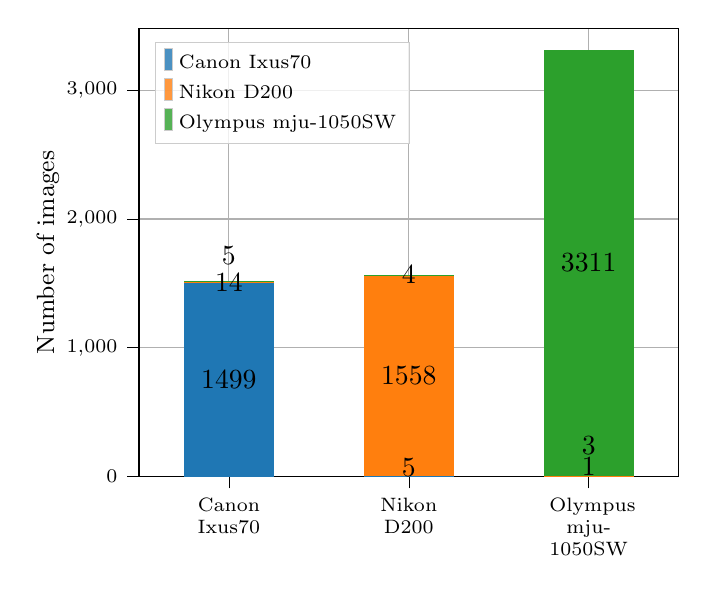
\begin{tikzpicture}

\definecolor{color0}{rgb}{0.12156862745098,0.466666666666667,0.705882352941177}
\definecolor{color1}{rgb}{1,0.498039215686275,0.0549019607843137}
\definecolor{color2}{rgb}{0.172549019607843,0.627450980392157,0.172549019607843}

\pgfplotsset{compat=1.11,
	/pgfplots/ybar legend/.style={
		/pgfplots/legend image code/.code={%
			\draw[##1,/tikz/.cd,yshift=-0.25em]
			(0cm,0cm) rectangle (3pt,0.8em);},
	}, every tick label/.append style={font=\scriptsize}
}

\begin{axis}[
legend cell align={left},
legend style={fill opacity=0.8, draw opacity=1, text opacity=1, at={(0.03,0.97)}, anchor=north west, draw=white!80!black},
tick align=outside,
tick pos=left,
grid=major,
x grid style={white!69.0196078431373!black},
xmin=-0.5, xmax=2.5,
xtick style={color=black},
xtick={0,1,2},
xticklabel style={text width=1cm, align=center},
xticklabels={Canon Ixus70,Nikon D200,Olympus mju-1050SW},
y grid style={white!69.0196078431373!black},
ymin=0, ymax=3480.75,
ytick style={color=black},
y label style={at={(axis description cs:-0.13,.5)},anchor=south},
ylabel={\small Number of images}
]
\draw[draw=none,fill=color0] (axis cs:-0.25,0) rectangle (axis cs:0.25,1499);
\addlegendimage{ybar,ybar legend,draw=none,fill=color0};
\addlegendentry{\scriptsize Canon Ixus70}

\draw[draw=none,fill=color0] (axis cs:0.75,0) rectangle (axis cs:1.25,5);
\draw[draw=none,fill=color0] (axis cs:1.75,0) rectangle (axis cs:2.25,1);
\draw[draw=none,fill=color1] (axis cs:-0.25,1499) rectangle (axis cs:0.25,1513);
\addlegendimage{ybar,ybar legend,draw=none,fill=color1};
\addlegendentry{\scriptsize Nikon D200}

\draw[draw=none,fill=color1] (axis cs:0.75,5) rectangle (axis cs:1.25,1563);
\draw[draw=none,fill=color1] (axis cs:1.75,1) rectangle (axis cs:2.25,4);
\draw[draw=none,fill=color2] (axis cs:-0.25,1513) rectangle (axis cs:0.25,1518);
\addlegendimage{ybar,ybar legend,draw=none,fill=color2};
\addlegendentry{\scriptsize Olympus mju-1050SW}

\draw[draw=none,fill=color2] (axis cs:0.75,1563) rectangle (axis cs:1.25,1567);
\draw[draw=none,fill=color2] (axis cs:1.75,4) rectangle (axis cs:2.25,3315);
\draw (axis cs:0,749.5) node[
  scale=1,
  text=black,
  rotate=0.0
]{1499};
\draw (axis cs:1,70) node[
  scale=1,
  text=black,
  rotate=0.0
]{5};
\draw (axis cs:2,80) node[
  scale=1,
  text=black,
  rotate=0.0
]{1};
\draw (axis cs:0,1506) node[
  scale=1,
  text=black,
  rotate=0.0
]{14};
\draw (axis cs:1,784) node[
  scale=1,
  text=black,
  rotate=0.0
]{1558};
\draw (axis cs:2,240) node[
  scale=1,
  text=black,
  rotate=0.0
]{3};
\draw (axis cs:0,1715) node[
  scale=1,
  text=black,
  rotate=0.0
]{5};
\draw (axis cs:1,1565) node[
  scale=1,
  text=black,
  rotate=0.0
]{4};
\draw (axis cs:2,1659.5) node[
  scale=1,
  text=black,
  rotate=0.0
]{3311};
\end{axis}

\end{tikzpicture}
